\chapter{HASIL DAN PEMBAHASAN}
\label{chap:hasil dan pembahasan}

% Ubah bagian-bagian berikut dengan isi dari pengujian dan analisis
\thispagestyle{newchap}

\section{Hasil Data \textit{Ground Test}}
Hasil pengukuran data \textit{ground test} dibagi menjadi 2 bagian, seperti yang telah dijelaskan pada bagian metodologi penelitian (BAB \ref{chap:metodologipenelitian}), bahwa data yang didapatkan merupakan data pengukuran getaran pada FTIS untuk mencari \textit{damping ratio} dan pengukuran data getaran pada akseleromter untuk mendapatkan respon frekuensi dominan oleh helikopter.

\subsection{Hasil Pengukuran Data Vibrasi pada FTIS}
\label{FTIS}

\begin{figure}[H]
	\begin{subfigure}{0.45\textwidth}
		\centering
		\includegraphics[width=\linewidth]{gambar/Lateral_input.png}
		\caption{}
		\label{fig:Lateral_input}
	\end{subfigure}
	\centering
	\begin{subfigure}{0.45\textwidth}
		\centering
		\includegraphics[width=\linewidth]{gambar/Lateral_output.png}
		\caption{}
		\label{fig:Lateral_output}
	\end{subfigure}
	\caption{Data hasil pengukuran menggunakan FTIS kondisi-1 (a) \textit{Input lateral}. (b) Respon terhadap \textit{output} linier oleh \textit{input lateral}.}
	\label{fig:io_lat}
\end{figure}

\begin{figure}[H]
	\begin{subfigure}{0.45\textwidth}
		\centering
		\includegraphics[width=\linewidth]{gambar/Longitudinal_input.png}
		\caption{}
		\label{fig:Longitudinal_input}
	\end{subfigure}
	\centering
	\begin{subfigure}{0.45\textwidth}
		\centering
		\includegraphics[width=\linewidth]{gambar/Longitudinal_output.png}
		\caption{}
		\label{fig:Longitudinal_output}
	\end{subfigure}
	\caption{Data hasil pengukuran menggunakan FTIS kondisi-1 (a) \textit{Input longitudinal}. (b) Respon terhadap \textit{output} linier oleh \textit{input longitudinal}.}
	\label{fig:io_long}
\end{figure}

\begin{figure}[H]
	\begin{subfigure}{0.45\textwidth}
		\centering
		\includegraphics[width=\linewidth]{gambar/Pedal_input.png}
		\caption{}
		\label{fig:Pedal_input}
	\end{subfigure}
	\centering
	\begin{subfigure}{0.45\textwidth}
		\centering
		\includegraphics[width=\linewidth]{gambar/Pedal_output.png}
		\caption{}
		\label{fig:Pedal_output}
	\end{subfigure}
	\caption{Data hasil pengukuran menggunakan FTIS kondisi-1 (a) \textit{Input Pedal}. (b) Respon terhadap \textit{output} linier oleh \textit{input Pedal}.}
	\label{fig:io_pedal}
\end{figure}

Gambar \ref{fig:io_lat} merupakan grafik \textit{input lateral} dan responnya pada \textit{roll, rate of roll} dan percepatan di sumbu-x. Kemudian pada gambar \ref{fig:io_long} merupakan grafik \textit{input longitudinal} dan responnya pada \textit{pitch, rate of pitch} dan percepatan di sumbu-y. Sedangkan pada gambar \ref{fig:io_pedal} merupakan grafik \textit{input pedal} dan responnya \textit{heading, rate of yaw} dan percepatan pada sumbu-z. Ketiga gambar tersebut, didapatkan dari hasil pengukuran FTIS sesuai pada variasi kondisi (tabel \ref{tb:variasilanding}) dan variasi \textit{input} (tabel \ref{tb:variasi_input}). Hasil keseluruhan data yang didapatkan menggunakan FTIS merupakan gabungan dari gambar \ref{fig:io_lat}, \ref{fig:io_long}, dan \ref{fig:io_pedal}. Sehingga secara keseluruhan, penyajian informasi berupa grafik tersebut dapat dilihat pada gambar \ref{fig:condition_1}.

\begin{figure}[H]
	\centering
	\includegraphics[width=\linewidth]{gambar/Config_1_all.png}
	\caption{Data hasil keseluruhan pengukuran menggunakan FTIS kondisi-1.}
	\label{fig:condition_1}
\end{figure}

Data pengukuran menggunakan FTIS sesuai dengan metodologi yang diberikan pada BAB \ref{chap:metodologipenelitian} dengan variasi kondisi pengukuran pada tabel \ref{tb:variasilanding} disajikan dalam beberapa grafik sekaligus yang berisi \textit{input} dan \textit{output}. Salah satu data hasil pengujian tersebut dapat dilihat pada gambar \ref{fig:condition_1}. Dimana pada gambar tersebut merupakan data hasil pengujian menggunakan FTIS pada kondisi-1.

Pada gambar \ref{fig:condition_1} \textit{input} \textit{lateral} dan \textit{longitudinal} secara bergantian memberikan pengaruh terhadap \textit{output} helikopter. Respon \textit{output} pada helikopter saat diberikan \textit{input} diidentifikasi seperti pada gambar \ref{fig:condition_1_identify}. Identifikasi dilakukan secara visual untuk selanjutnya dapat dihitung nilai \textit{logarithmic decrement} dan \textit{damping ratio} nya dengan menggunakan formulasi pada persamaan \ref{eq:logdec} dan \ref{eq:damp_ratio}.

\begin{figure}[H]
	\centering
	\includegraphics[width=0.8\linewidth]{gambar/Config_1_all_identify.png}
	\caption{Identifikasi \textit{input} dan \textit{output} hasil data pengukuran pada FTIS kondisi-1.}
	\label{fig:condition_1_identify}
\end{figure}

\begin{figure}[H]
	\centering
	\includegraphics[width=0.8\linewidth]{gambar/Config_1_all_identify_zoom_marker_7.png}
	\caption{Identifikasi secara visual saat helikopter masih memberikan respon setelah \textit{input} nya berhenti pada kondisi-1.}
	\label{fig:condition_1_identify_calc}
\end{figure}

Gambar \ref{fig:condition_1_identify_calc} merupakan hasil perbesaran tampilan data pengukuran dari area yang berwarna merah pada gambar \ref{fig:condition_1_identify}. Pada gambar \ref{fig:condition_1_identify_calc} menggambarkan kondisi saat \textit{input lateral} diberikan dan terdapat respon pada setiap \textit{outputnya}. Sehingga dari gambar \ref{fig:condition_1_identify_calc} akan dilakukan identifikasi melalui contoh perhitungan untuk mencari \textit{logarithmic decrement} dan \textit{damping ratio}.

Daerah hijau pada gambar \ref{fig:condition_1_identify_calc} merupakan rentang saat \textit{input} pada helikopter telah berhenti. Namun, pada bagian \textit{output} nya masih memberikan respon, yaitu pada \textit{rate of roll} dan percepatan pada sumbu-y. Sehingga pada \textit{output} tersebut selanjutnya akan diidentifikasi secara visual untuk kemudian dihitung besarnya \textit{logarithmic decrement} dan \textit{damping ratio} nya.

\begin{figure}[H]
	\centering 
	\begin{subfigure}{0.48\textwidth}
		\centering
		\includegraphics[width=\linewidth]{gambar/Config_1_ROR.png}
		\caption{}
		\label{fig:condition_1_ROR}
	\end{subfigure}
	\centering
	\begin{subfigure}{0.48\textwidth}
		\centering
		\includegraphics[width=\linewidth]{gambar/Config_1_acc-y.png}
		\caption{}
		\label{fig:condition_1_acc-y}	
	\end{subfigure}
	\caption{Identifikasi secara visual saat helikopter masih memberikan respon setelah \textit{input} nya berhenti pada kondisi-1 data hasil pengukuran dengan FTIS: (a) Respon \textit{rate of roll} (deg/s). (b) Respon pada percepatan sumbu-y (m/s$^2$).}
	\label{fig:identifikasi_config1}
\end{figure}

Sebagai contoh perhitungan, pada gambar \ref{fig:condition_1_ROR} digunakan persamaan \ref{eq:logdec}, didapatkan $x_{m+1}$ memiliki nilai sebesar 0.8 dan $x_1$ sebesar 0.2, dengan $m$ sebanyak 5 puncak maka didapatkan besarnya \textit{logarithmic decrement} sebesar 0.27. Nilai tersebut apabila dimasukkan pada persamaan \ref{eq:damp_ratio} maka akan didapatkan besarnya \textit{damping ratio} sebesar 0.044. Dengan cara yang sama, maka akan didapatkan besarnya \textit{logarithmic decrement} dan \textit{damping ratio} pada respon percepatan sumbu-y (gambar \ref{fig:condition_1_acc-y}) berturut-turut adalah sebesar 0.34 dan 0.055. Untuk semua respon pada setiap kondisi yang didefinisikan pada tabel \ref{tb:variasilanding} dengan variasi \textit{input} dari tabel \ref{tb:variasi_input} dilakukan cara perhitungan yang sama seperti menghitung \textit{logarithmic decrement} dan \textit{damping ratio} pada gambar \ref{fig:identifikasi_config1}.

Tidak semua respon dapat dihitung besarnya \textit{logarithmic decrement} dan \textit{damping ratio} nya, hal itu dikarenakan responnya tidak lagi memberikan nilai setelah \textit{input} berhenti diberikan oleh helikopter. Respon tersebut terdapat pada gambar \ref{fig:condition_1_identify_calc} ditandai dengan lingkaran bergaris merah, dimana pada respon \textit{rate of pitch}, \textit{rate of yaw}, percepatan sumbu-x dan percepatan sumbu-z tidak terdapat respon setelah \textit{input} berhenti. Sedangkan untuk respon pada \textit{roll}, \textit{pitch} dan \textit{heading} bahkan tidak memiliki respon yang cukup untuk diidentifikasi saat \textit{input} masih diberikan pada helikopter.

Berdasarkan tabel \ref{tb:variasilanding} kondisi-1 merupakan kondisi saat semua tekanan pada ban-oleo di bagian badan helikopter berada pada tekanan yang normal (\textit{nominal}). Sedangkan kondisi-6 saat semua tekanan pada ban-oleo di bagian badan helikopter berada pada tekanan tinggi (\textit{high}) dan kondisi-7 saat semua tekanannya rendah (\textit{low}). Sehingga kemudian dari ketiga kondisi tersebut (1, 6 dan 7) akan menjadi bagian dari pembahasan terhadap variasi besaran tekanan.

\begin{figure}[H]
	\centering
	\begin{subfigure}{0.48\textwidth}
		\centering
		\includegraphics[width=\linewidth]{gambar/ROR_bar.png}
		\caption{}
		\label{fig:ROR_1,6,7}
	\end{subfigure}
	\centering
	\begin{subfigure}{0.48\textwidth}
		\centering
		\includegraphics[width=\linewidth]{gambar/ROP_bar.png}
		\caption{}
		\label{fig:ROP_1,6,7}
	\end{subfigure}
	\\
	\centering
	\begin{subfigure}{0.48\textwidth}
		\centering
		\includegraphics[width=\linewidth]{gambar/ROY_bar.png}
		\caption{}
		\label{fig:ROY_1,6,7}
	\end{subfigure}
	\centering
	\begin{subfigure}{0.48\textwidth}
		\centering
		\includegraphics[width=\linewidth]{gambar/ACC-Y_bar.png}
		\caption{}
		\label{fig:ACC-y_1,6,7}
	\end{subfigure}
		\caption{Besarnya \textit{damping ratio} untuk kondisi-7 (\textit{low}), kondisi-1 (\textit{nominal}) dan kondisi-6 (\textit{high}) pada respon (a) \textit{rate of roll}, (b) \textit{rate of pitch}, (c) \textit{rate of yaw} dan (d) percepatan pada sumbu-y.}
		\label{fig:damp_ratio_1,6,7}
\end{figure}

Grafik yang disajikan pada gambar \ref{fig:damp_ratio_1,6,7} merupakan besarnya nilai \textit{damping ratio} yang didapatkan melalui perhitungan yang sama saat menghitung \textit{damping ratio} pada kondisi-1 di gambar \ref{fig:identifikasi_config1}. Pada gambar \ref{fig:damp_ratio_1,6,7}, untuk respon \textit{rate of pitch} dan percepatan arah sumbu-y, \textit{damping ratio} dari keadaan '\textit{nominal}' memiliki nilai yang relatif lebih rendah dibandingkan dua kondisi lainnya. Sedangkan untuk respon \textit{rate of roll}, nilai \textit{damping ratio} dari keadaan '\textit{nominal}' sedikit lebih besar dari dua kondisi lainnya ('\textit{low}' dan '\textit{high}'). Disisi lain, respon \textit{rate of yaw} hanya dapat diidentifikasi dari keadaan '\textit{low}' dan tidak terdapat respon dari keadaan saat '\textit{nominal}' dan '\textit{high}'.

Selanjutnya, untuk semua kondisi yang telah didefinisikan pada tabel \ref{tb:variasilanding} telah dihitung menggunakan perhitungan yang sama, yaitu menggunakan persamaan \ref{eq:logdec}, didapatkan rata-rata total dari masing-masing kondisi. Informasi terkait besaran tersebut dapat dilihat pada tabel \ref{tb:damp_ratio_table}. 

\begin{table}[H]
	\centering
	\caption{Hasil identifikasi damping ratio rata-rata dari respon helikopter berdasarkan variasi kondisi.}
	\label{tb:damp_ratio_table}
	\resizebox{\textwidth}{!}{%
		\begin{tabular}{|c|ccccccccc|}
			\hline
			\multirow{2}{*}{Kondisi ke-} & \multicolumn{9}{c|}{Rata-rata \textit{damping ratio} respon} \\ \cline{2-10} 
			& \multicolumn{1}{c|}{Roll} & \multicolumn{1}{c|}{Pitch} & \multicolumn{1}{c|}{Heading} & \multicolumn{1}{c|}{Rate of Roll} & \multicolumn{1}{c|}{Rate of Pitch} & \multicolumn{1}{c|}{Rate of Yaw} & \multicolumn{1}{c|}{Acceleration-X} & \multicolumn{1}{c|}{Acceleration-Y} & Acceleration-Z \\ \hline
			1 & \multicolumn{1}{c|}{-} & \multicolumn{1}{c|}{-} & \multicolumn{1}{c|}{-} & \multicolumn{1}{c|}{0.05285435} & \multicolumn{1}{c|}{0.036747763} & \multicolumn{1}{c|}{-} & \multicolumn{1}{c|}{-} & \multicolumn{1}{c|}{0.050426643} & - \\ \hline
			2 & \multicolumn{1}{c|}{-} & \multicolumn{1}{c|}{-} & \multicolumn{1}{c|}{-} & \multicolumn{1}{c|}{0.058120539} & \multicolumn{1}{c|}{-} & \multicolumn{1}{c|}{0.045805814} & \multicolumn{1}{c|}{-} & \multicolumn{1}{c|}{0.038387333} & - \\ \hline
			3 & \multicolumn{1}{c|}{-} & \multicolumn{1}{c|}{-} & \multicolumn{1}{c|}{-} & \multicolumn{1}{c|}{0.055225124} & \multicolumn{1}{c|}{0.05507518} & \multicolumn{1}{c|}{0.043144563} & \multicolumn{1}{c|}{-} & \multicolumn{1}{c|}{0.040316101} & - \\ \hline
			4 & \multicolumn{1}{c|}{-} & \multicolumn{1}{c|}{-} & \multicolumn{1}{c|}{-} & \multicolumn{1}{c|}{0.055248847} & \multicolumn{1}{c|}{0.04408422} & \multicolumn{1}{c|}{0.036747763} & \multicolumn{1}{c|}{-} & \multicolumn{1}{c|}{0.062462147} & - \\ \hline
			5 & \multicolumn{1}{c|}{-} & \multicolumn{1}{c|}{-} & \multicolumn{1}{c|}{-} & \multicolumn{1}{c|}{0.064958942} & \multicolumn{1}{c|}{0.054761252} & \multicolumn{1}{c|}{-} & \multicolumn{1}{c|}{-} & \multicolumn{1}{c|}{0.035288539} & - \\ \hline
			6 & \multicolumn{1}{c|}{-} & \multicolumn{1}{c|}{-} & \multicolumn{1}{c|}{-} & \multicolumn{1}{c|}{0.050658456} & \multicolumn{1}{c|}{0.04408422} & \multicolumn{1}{c|}{-} & \multicolumn{1}{c|}{-} & \multicolumn{1}{c|}{0.064120389} & - \\ \hline
			7 & \multicolumn{1}{c|}{-} & \multicolumn{1}{c|}{-} & \multicolumn{1}{c|}{-} & \multicolumn{1}{c|}{0.04732238} & \multicolumn{1}{c|}{0.043670692} & \multicolumn{1}{c|}{0.047821495} & \multicolumn{1}{c|}{-} & \multicolumn{1}{c|}{0.064757723} & - \\ \hline
			8 & \multicolumn{1}{c|}{-} & \multicolumn{1}{c|}{-} & \multicolumn{1}{c|}{-} & \multicolumn{1}{c|}{0.049504081} & \multicolumn{1}{c|}{0.05727551} & \multicolumn{1}{c|}{-} & \multicolumn{1}{c|}{-} & \multicolumn{1}{c|}{0.048365129} & - \\ \hline
			9 & \multicolumn{1}{c|}{-} & \multicolumn{1}{c|}{-} & \multicolumn{1}{c|}{-} & \multicolumn{1}{c|}{-} & \multicolumn{1}{c|}{-} & \multicolumn{1}{c|}{-} & \multicolumn{1}{c|}{-} & \multicolumn{1}{c|}{-} & - \\ \hline
			10 & \multicolumn{1}{c|}{-} & \multicolumn{1}{c|}{-} & \multicolumn{1}{c|}{-} & \multicolumn{1}{c|}{-} & \multicolumn{1}{c|}{-} & \multicolumn{1}{c|}{-} & \multicolumn{1}{c|}{-} & \multicolumn{1}{c|}{-} & - \\ \hline
			11 & \multicolumn{1}{c|}{-} & \multicolumn{1}{c|}{-} & \multicolumn{1}{c|}{-} & \multicolumn{1}{c|}{-} & \multicolumn{1}{c|}{-} & \multicolumn{1}{c|}{-} & \multicolumn{1}{c|}{-} & \multicolumn{1}{c|}{-} & - \\ \hline
			Rata-rata total & \multicolumn{1}{c|}{-} & \multicolumn{1}{c|}{-} & \multicolumn{1}{c|}{-} & \multicolumn{1}{c|}{0.05423659} & \multicolumn{1}{c|}{0.047956977} & \multicolumn{1}{c|}{0.043379909} & \multicolumn{1}{c|}{-} & \multicolumn{1}{c|}{0.050515501} & - \\ \hline
		\end{tabular}%
	}
\end{table}

\begin{figure}[H]
	\centering
	\includegraphics[width=0.75\linewidth]{gambar/damp_motion_heli.png}
	\caption{Identifikasi secara visual saat helikopter masih memberikan respon setelah \textit{input} nya berhenti pada kondisi-1.}
	\label{fig:damp_motion_heli}
\end{figure}

Pada tabel \ref{tb:damp_ratio_table}, tidak ditemukan besarnya \textit{damping ratio} pada respon \textit{roll}, \textit{pitch}, \textit{heading}, percepatan pada sumbu-x dan sumbu-z. Hal tersebut karena tidak ditemukan adanya respon yang dapat diidentifikasi secara visual. Dengan kata lain, helikopter tidak memiliki respon percepatan pada arah sumbu-x dan sumbu-z. Dari tabel \ref{tb:damp_ratio_table}, nilai \textit{damping ratio} rata-rata terkecil berasal dari respon \textit{rate of yaw} (0.043) dan \textit{rate of pitch} (0.047) dibandingkan dengan respon \textit{rate of roll} (0.054) dan respon percepatan pada arah sumbu-y (0.050). Nilai \textit{damping ratio} pada tabel \ref{tb:damp_ratio_table} dan pada gambar \ref{fig:damp_motion_heli} menunjukkan bahwa, helikopter cenderung memiliki getaran pada arah beloknya (kanan-kiri) serta getaran pada arah \textit{pitch} (rotasi depan-belakang).

\subsection{Hasil Pengukuran Data Vibrasi Akselerometer}

Data yang didapatkan dari hasil sensor akselerometer ditunjukkan pada gambar dibawah ini:

\begin{figure}[h]
	\centering
	\includegraphics[width=0.7\linewidth]{gambar/raw_config2_ch1.png}
	\caption{Grafik data pengukuran pada variasi FILO kondisi-2 \textit{channel} 1.}
	\label{fig:raw_config2_FILO}
\end{figure}

\begin{figure}[H]
	\centering
	\includegraphics[width=0.7\linewidth]{gambar/fft_config2_ch1.png}
	\caption{Grafik data hasil FFT pada variasi FILO kondisi-2.}
	\label{fig:fft_config2_FILO}
\end{figure}

Grafik pada gambar \ref{fig:raw_config2_FILO} merupakan grafik data hasil pengukuran yang didapatkan oleh sensor akselerometer pada \textit{channel} 1 dan grafik pada \ref{fig:fft_config2_FILO} merupakan grafik data yang telah diolah menggunakan FFT, sehingga didapatkan nilai dalam domain frekuensi. Data hasil pengukuran menggunakan akselerometer pada gambar diatas akan dibandingkan dengan acuan dari MIL-STD-810H-Method-514.8 (vibrasi) \cite{MILSTD}. Standar tersebut pada dasarnya digunakan sebagai alternatif pengganti \textit{ground vibration test} (GVT) seperti yang dilakukan pada \cite{lubrina:hal-01059708} dan \cite{Ciavarella2018AnEH}. Informasi dari tabel \ref{tb:batas_siklus} didapatkan batas siklus osilasi helikopter. Sehingga dapat dihasilkan grafik batas siklus osilasi pada gambar \ref{fig:batas_siklus}. 

\begin{figure}[h]
	\centering
	\includegraphics[width=0.75\linewidth]{gambar/Oscillation_cycle_limit.jpg}
	\caption{Grafik batas siklus osilasi dari acuan MIL-STD-810H-Method-514.8 (vibrasi).}
	\label{fig:batas_siklus}
\end{figure}

\begin{table}[]
	\centering
	\caption{Tabel perhitungan batas siklus osilasi.}
	\label{tb:batas_siklus}
	\resizebox{0.8\textwidth}{!}{%
		\begin{tabular}{|ccc|c|ccc|}
			\hline
			\multicolumn{3}{|c|}{Frequency (Hz)} & Frekuensi harmonik & \multicolumn{3}{c|}{Peak (g)} \\ \hline
			\multicolumn{1}{|c|}{\multirow{2}{*}{$f_1$}} & \multicolumn{1}{c|}{lower} & 5.92 & \multirow{2}{*}{1p} & \multicolumn{1}{c|}{\multirow{2}{*}{$A_1$}} & \multicolumn{1}{c|}{lower} & 0.146443515 \\ \cline{2-3} \cline{6-7} 
			\multicolumn{1}{|c|}{} & \multicolumn{1}{c|}{upper} & 6.08 &  & \multicolumn{1}{c|}{} & \multicolumn{1}{c|}{upper} & 0.151515152 \\ \hline
			\multicolumn{1}{|c|}{\multirow{2}{*}{$f_2$}} & \multicolumn{1}{c|}{lower} & 23.68 & \multirow{2}{*}{1p*n} & \multicolumn{1}{c|}{\multirow{2}{*}{$A_2$}} & \multicolumn{1}{c|}{lower} & 2.368 \\ \cline{2-3} \cline{6-7} 
			\multicolumn{1}{|c|}{} & \multicolumn{1}{c|}{upper} & 24.32 &  & \multicolumn{1}{c|}{} & \multicolumn{1}{c|}{upper} & 2.432 \\ \hline
			\multicolumn{1}{|c|}{\multirow{2}{*}{$f_3$}} & \multicolumn{1}{c|}{lower} & 47.36 & \multirow{2}{*}{1p*n*2} & \multicolumn{1}{c|}{\multirow{2}{*}{$A_3$}} & \multicolumn{1}{c|}{lower} & 1.764 \\ \cline{2-3} \cline{6-7} 
			\multicolumn{1}{|c|}{} & \multicolumn{1}{c|}{upper} & 48.64 &  & \multicolumn{1}{c|}{} & \multicolumn{1}{c|}{upper} & 1.636 \\ \hline
			\multicolumn{1}{|c|}{\multirow{2}{*}{$f_4$}} & \multicolumn{1}{c|}{lower} & 71.04 & \multirow{2}{*}{1p*n*3} & \multicolumn{1}{c|}{\multirow{2}{*}{$A_4$}} & \multicolumn{1}{c|}{lower} & 1.5 \\ \cline{2-3} \cline{6-7} 
			\multicolumn{1}{|c|}{} & \multicolumn{1}{c|}{upper} & 72.96 &  & \multicolumn{1}{c|}{} & \multicolumn{1}{c|}{upper} & 1.5 \\ \hline
		\end{tabular}%
	}
\end{table}

Untuk mendapatkan grafik pada gambar \ref{fig:batas_siklus} diperlukan informasi kecepatan rotor helikopter. Diketahui (informasi \textit{flight manual} dari PTDI) nilai kecepatan maksimum dan minimum dari rotor berturut-turut adalah sebesar $365 rpm$ dan $355 rpm$, sehingga didapatkan frekuensi ($f_1$) nya dimulai dari 5.92Hz (minimum) hingga 6.08Hz (maksimum). Perhitungan nilai $f_2$, $f_3$, dan $f_4$ dapat dilihat pada tabel \ref{tb:batas_siklus}. Nilai peak pada tabel tersebut dihitung menggunakan formulasi pada tabel \ref{tb:MIL-STD} yang terletak pada kolom "\textbf{PEAK ACCELERATION ($A_x$) at $f_x$ (GRAVITY UNITS (g))}". Berdasarkan standar yang dimiliki oleh \cite{MILSTD} terdapatnya nilai respon frekuensi pada batas siklus osilasi menunjukkan potensi kejadian terburuk (salah satunya adalah fenomena \textit{ground resonance}) yang secara langsung akan berkaitan dengan keselamatan dan kelayakan penerbangan helikopter. Namun, dari respon yang diberikan oleh helikopter pada semua variasi kondisi dan \textit{input} nilai puncak tertinggi yang dimiliki oleh respon helikopter hanya berada pada nilai 0.143 pada $f_2$ yaitu 23.68 hingga 24.32Hz. Sehingga, dari grafik pada gambar \ref{fig:11_FLLO} (kondisi-11 variasi FLLO) tidak ditemukan potensi adanya \textit{ground resonance} pada helikopter. Adapun respon pada kondisi yang lain dengan variasi \textit{input} yang telah ditentukan, responnya memiliki nilai yang lebih kecil dari kondisi pada gambar \ref{fig:11_FLLO}, meskipun respon tersebut berada pada batas siklus osilasi helikopter.

\begin{figure}[h]
	\centering
	\includegraphics[width=0.5\linewidth]{gambar/Helicopter_response_GVT_image/Config_11/5_Config_11_FLLO.jpg}
	\caption{Hasil pengukuran respon frekuensi kondisi-11 pada variasi FLLO pada detik 1800-1850.}
	\label{fig:11_FLLO}
\end{figure}

Grafik pada gambar \ref{fig:11_FLLO} merupakan contoh grafik dengan nilai respon terbesar dibandingkan respon-respon dari kondisi dan variasi lainnya, yaitu dengan amplitudo sebesar 0.143 g-peak pada frekuensi 23.74Hz. Nilai respon yang diberikan pada grafik tersebut merupakan nilai yang didapatkan dari \textit{channel} 1 hingga 6. Data respon yang diberi tanda 'x' merupakan nilai tertinggi dari grafik FFT yang telah didapatkan. Selanjutnya akan coba diidentifikasi bagaimana respon helikopter pada masing-masing \textit{channel} yang dimulai dari \textit{channel}-1 hingga 6 untuk semua kondisi.

\begin{figure}[H]
	\centering
	\includegraphics[width=0.5\linewidth]{gambar/Plot_per_channel_FTIS/all_channel_1.jpg}
	\caption{Hasil pengukuran respon frekuensi pada \textit{channel} 1 (arah sumbu-z) untuk semua kondisi.}
	\label{fig:channel_1}
\end{figure}

\begin{figure}[h]
	\centering
	\includegraphics[width=0.5\linewidth]{gambar/Plot_per_channel_FTIS/all_channel_2.jpg}
	\caption{Hasil pengukuran respon frekuensi pada \textit{channel} 2 (arah sumbu-z) untuk semua kondisi.}
	\label{fig:channel_2}
\end{figure}

\begin{figure}[]
	\centering
	\includegraphics[width=0.5\linewidth]{gambar/Plot_per_channel_FTIS/all_channel_3.jpg}
	\caption{Hasil pengukuran respon frekuensi pada \textit{channel} 3 (arah sumbu-y) untuk semua kondisi.}
	\label{fig:channel_3}
\end{figure}

\begin{figure}[H]
	\centering
	\includegraphics[width=0.5\linewidth]{gambar/Plot_per_channel_FTIS/all_channel_4.jpg}
	\caption{Hasil pengukuran respon frekuensi pada \textit{channel} 4 (arah sumbu-z) untuk semua kondisi.}
	\label{fig:channel_4}
\end{figure}

\begin{figure}[h]
	\centering
	\includegraphics[width=0.5\linewidth]{gambar/Plot_per_channel_FTIS/all_channel_5.jpg}
	\caption{Hasil pengukuran respon frekuensi pada \textit{channel} 5 (arah sumbu-x) untuk semua kondisi.}
	\label{fig:channel_5}
\end{figure}

\begin{figure}[H]
	\centering
	\includegraphics[width=0.5\linewidth]{gambar/Plot_per_channel_FTIS/all_channel_6.jpg}
	\caption{Hasil pengukuran respon frekuensi pada \textit{channel} 6 (arah sumbu-y) untuk semua kondisi.}
	\label{fig:channel_6}
\end{figure}

Grafik pada gambar \ref{fig:channel_1} hingga \ref{fig:channel_6} memberikan informasi terkait respon helikopter dari \textit{channel} 1 hingga 6 untuk semua kondisi. Respon helikopter bertanda 'x' dan diberi warna hijau. Respon tersebut lebih banyak terdapat pada sekitar batas siklus di $f_1$ dan $f_2$. Akan tetapi berdasarkan data yang telah diolah, tidak terdapat respon helikopter yang berada pada batas siklus $f_1$ hal ini dibuktikan dengan identifikasi nilai kuantitatif respon pada interval $f_1$ seperti yang terdapat pada tabel \ref{tb:identifikasi_pada_batas_siklus} dan tabel \ref{tab:jumlah_proporsi_respon_frekuensi}. Dari tabel tersebut, terdapat sebanyak 15.87$\%$ respon helikopter pada batas siklus $f_2$, 4.27$\%$ pada batas siklus $f_3$ dan 0.621$\%$ pada batas siklus $f_4$, sedangkan didapatkan total respon yang berada pada batas siklus hanya sebesar 20.77$\%$ dari total respon yang berada pada rentang 0-80Hz. 

\begin{figure}[H]
	\centering
	\includegraphics[width=0.84\linewidth]{gambar/respon_tampak_atas.png}
	\caption{Proporsi respon frekuensi pada helikopter untuk masing-masing \textit{channel} beserta arah orientasi akselerometer.}
	\label{fig:respon_tampak_atas}
\end{figure}

Gambar \ref{fig:respon_tampak_atas} memberikan informasi terkait proporsi getaran yang diberikan oleh helikopter terhadap input yang diberikan oleh masing-masing \textit{channel}. \textit{Channel} 1,2, dan 3 tidak memberikan informasi terhadap pergerakan sumbu-x. Namun, didapatkan respon pada \textit{channel}-6 bernilai lebih besar dibandingkan respon pada \textit{channel}-3, hal ini memberikan informasi bahwa pada titik 3 dengan arah sumbu-y lebih sering didapati respon getaran dibandingkan dengan titik 2. Hal ini kemudian dapat diartikan bahwa helikopter memiliki gerakan arah kanan dan kiri. Disisi lain, respon getaran pada sumbu-z di titik 3 memiliki jumlah respon yang lebih banyak dikarenakan helikopter memiliki kecenderungan bergerak ke-arah \textit{pitch} depan dan belakang seperti yang telah dijelaskan pada bagian \ref{FTIS}. Sehingga, helikopter lebih cenderung memberikan respon Getaran dengan arah sumbu-y dan arah kanan-kiri terhadap orientasinya. 

\begin{table}[H]
	\centering
	\caption{Persentase banyaknya respon Helikopter pada batas siklus osilasi.}
	\label{tb:identifikasi_pada_batas_siklus}
	\resizebox{0.5\textwidth}{!}{%
		\begin{tabular}{|cc|c|}
			\hline
			\multicolumn{1}{|c|}{Batas Siklus} & Banyak respon (n) & Proporsi respon (\%) \\ \hline
			\multicolumn{1}{|c|}{$f_1$} & 0 & 0.00 \\ \hline
			\multicolumn{1}{|c|}{$f_2$} & 383 & 15.88 \\ \hline
			\multicolumn{1}{|c|}{$f_3$} & 103 & 4.27 \\ \hline
			\multicolumn{1}{|c|}{$f_4$} & 15 & 0.62 \\ \hline
			\multicolumn{2}{|c|}{Total proporsi respon (\%)} & 20.77 \\ \hline
		\end{tabular}%
	}
\end{table}

\begin{table}[H]
	\centering
	\caption{Persentase banyaknya respon helikopter pada batas siklus osilasi berdasarkan masing-masing channel.}
	\label{tab:jumlah_proporsi_respon_frekuensi}
	\resizebox{\textwidth}{!}{%
		\begin{tabular}{|c|c|c|c|c|
				>{\columncolor[HTML]{FFCE93}}c |
				>{\columncolor[HTML]{FFCB2F}}c 
				>{\columncolor[HTML]{FFCB2F}}l |}
			\hline
			\textit{Channel} & $f_1$ (n) & $f_2$ (n) & $f_3$ (n) & $f_4$ (n) & Total per \textit{channel} & \multicolumn{2}{c|}{\cellcolor[HTML]{FFCB2F}Proporsi masing-masing \textit{channel} (\%)} \\ \hline
			ch1 & 0 & 97 & 25 & 4 & 126 & \multicolumn{2}{c|}{\cellcolor[HTML]{FFCB2F}25.15} \\ \hline
			ch2 & 0 & 93 & 18 & 2 & 113 & \multicolumn{2}{c|}{\cellcolor[HTML]{FFCB2F}22.55} \\ \hline
			ch3 & 0 & 20 & 20 & 2 & 42 & \multicolumn{2}{c|}{\cellcolor[HTML]{FFCB2F}8.38} \\ \hline
			ch4 & 0 & 114 & 3 & 6 & 123 & \multicolumn{2}{c|}{\cellcolor[HTML]{FFCB2F}24.55} \\ \hline
			ch5 & 0 & 6 & 0 & 0 & 6 & \multicolumn{2}{c|}{\cellcolor[HTML]{FFCB2F}1.20} \\ \hline
			ch6 & 0 & 53 & 37 & 1 & 91 & \multicolumn{2}{c|}{\cellcolor[HTML]{FFCB2F}18.16} \\ \hline
			Total per batas siklus frekuensi & \cellcolor[HTML]{FFFE65}0 & \cellcolor[HTML]{FFFE65}383 & \cellcolor[HTML]{FFFE65}103 & \cellcolor[HTML]{FFFE65}15 & 501 & \multicolumn{2}{c|}{\cellcolor[HTML]{FFCB2F}100} \\ \hline
		\end{tabular}%
	}
\end{table}



Pada tabel \ref{tab:jumlah_proporsi_respon_frekuensi}, respon frekuensi yang berada pada batas siklus osilasi terbanyak ditemukan pada \textit{channel} 1, yaitu 25.15$\%$ kemudian pada \textit{channel} 4 sebesar 24.55$\%$, selanjutnya dari \textit{channel} 2 sebesar 22.55$\%$. Sisanya, yaitu dari \textit{channel} 6 dan 3 berturut-turut sebesar 18.16$\%$ dan 8.38$\%$. Adapun \textit{channel} yang paling sedikit memberikan respon frekuensi adalah pada \textit{channel} 5 yang memiliki orientasi pada arah sumbu-x yaitu sebesar 1.2$\%$. Hal ini menunjukkan bahwa pada helikopter lebih sedikit terjadi getaran yang bergerak ke-arah depan dan belakang helikopter.

\section{Hasil Perhitungan Matematis}

\subsection{Hasil Validasi Matematis}

Persamaan \ref{eq:EOM} yang ditampilkan dalam bentuk matriks memiliki 6 representatif gerakan \textit{degree of freedom} pada matriks \textbf{Q} pada persamaan \ref{eq:state-space}. Respon frekuensi helikopter pada arah sumbu-x direkonstruksi untuk dilakukan validasi pada persamaan matematika yang telah dibuat. Sehingga didapatkan grafik solusi dari persamaan \ref{eq:EOM} untuk gerak perpindahan pusat massa rotor $X_{G_r}(t)$ pada arah sumbu-x dan rekonstruksi respon frekuensi helikopter hasil pengukuran pada gambar \ref{fig:validation_time_domain}. 

\begin{figure}[H]
	\centering
	\includegraphics[width=\linewidth]{gambar/validation_time_domain.jpg}
	\caption{Respon frekuensi helikopter pada arah sumbu-x dan Plot persamaan matematis untuk solusi perpindahan pusat massa rotor pada arah sumbu-x.}
	\label{fig:validation_time_domain}
\end{figure}

Untuk memastikan bahwa respon hasil rekonstruksi sudah sesuai dengan data pengukuran, dilakukan FFT untuk melihat puncak pada respon hasil pengukuran dan respon hasil rekonstruksi. Respon hasil pengukuran dapat dilihat pada gambar \ref{fig:FFT_ch3} dan untuk FFT pada respon hasil rekonstruksi dan FFT solusi matematika dapat dilihat pada gambar \ref{fig:FFT_validation}.

\begin{figure}[H]
	\centering
	\includegraphics[width=0.8\linewidth]{gambar/FILA_9_FFT_ch3.png}
	\caption{Respon frekuensi helikopter pada arah sumbu-x dan Plot persamaan matematis untuk solusi perpindahan pusat massa rotor pada arah sumbu-x.}
	\label{fig:FFT_ch3}
\end{figure}

\begin{figure}[H]
	\centering
	\includegraphics[width=0.6\linewidth]{gambar/FILA_dummy_math.jpg}
	\caption{Grafik FFT data respon hasil rekonstruksi dan FFT dari solusi matematis perpindahan pusat massa rotor pada sumbu-x.}
	\label{fig:FFT_validation}
\end{figure}

\begin{figure}[H]
	\centering
	\includegraphics[width=0.8\linewidth]{gambar/measurement_solution.jpg}
	\caption{Grafik rekonstruksi respon hasil pengukuran dan solusi matematis pada arah sumbu-x Helikopter.}
	\label{fig:measur_solution}
\end{figure}


Dari gambar \ref{fig:FFT_ch3} dan \ref{fig:FFT_validation} didapatkan bahwa letak dominan frekuensi yang dihasilkan dari ketiga respon berada pada nilai yang berdekatan. Untuk hasil pengukuran didapatkan puncak (gambar \ref{fig:FFT_ch3}) berada pada frekuensi 16.334 Hz, 701.83 Hz, 748.285 Hz, dan 839.859 Hz. Sedangkan untuk FFT hasil rekonstruksi, responnya berada pada frekuensi 16.29 Hz, 701.9 Hz, 748.2 Hz dan 839.8 Hz. Sehingga respon hasil rekonstruksi dapat digunakan sebagai representatif hasil pengukuran.

Solusi persamaan yang telah dicantumkan pada gambar \ref{fig:validation_time_domain} setelah digunakan FFT, memiliki puncak pada frekuensi 16.72 Hz. Nilai error terdekat antara solusi persamaan matematis dan pengukuran berada pada nilai error 2.63$\%$. Sedangkan dari gambar \ref{fig:measur_solution} merupakan grafik yang menampilkan grafik solusi matematis untuk identifikasi error RMSE (\textit{Root Mean Square Error}) terhadap respon rekonstruksi hasil pengukuran. Dari hasil perhitungan komputasi pada Matlab didpatkan nilai RMSE nya adalah sebesar 0.017 atau sebesar 1.7$\%$.

Sehingga didapatkan secara matematis, pendekatan yang dilakukan merupakan pendekatan dengan besaran error perhitungan terhadap pengukuran sebesar 2.63$\%$ dalam domain frekuensinya. Salah satu faktor yang menyebabkan terjadinya error ini adalah penyederhanaan bentuk matematis yang banyak memberikan toleransi dalam identifikasinya. Disisi lain, pendekatan propertis mekanik yang masih kurang tepat dari kondisi pada bagian helikopter sebenarnya. Maka selanjutnya setelah diketahui besarnya error pada perhitungan matematis terhadap pengukuran, akan dilakukan analisis terhadap perhitungan matematis dan hasil pemodelan pada Femap.

\subsection{Analisis Matematis Ketidakstabilan Kondisi Normal}

Perhitungan matematis yang dilakukan berdasarkan dari apa yang telah dikerjakan pada \cite{BERGEOT201672}, frekuensi \textit{ground resonance} akan terjadi pada \textit{regressive rotor mode}, yaitu mode yang terjadi pada bilah rotor. Dalam perhitungan tersebut, digunakan matriks dari persamaan \ref{eq:state-space}. Berdasarkan matriks yang telah didapatkan pada persamaan \ref{eq:linearisasi} kemudian disubtitusi pada persamaan \ref{eq:EOM} dan diubah menjadi bentuk \textit{state-space} pada persamaan \ref{eq:state-space_simplified}, maka akan dihitung nilai eigen dari matriks \textbf{A}.

\begin{align*}
	\mathbf{A}=\begin{bmatrix}
	\mathbf{0}& \mathbf{I}\\
	\mathbf{-M}^{-1}\mathbf{K}& \mathbf{-M}^{-1}(\mathbf{C}+\mathbf{G})
	\end{bmatrix}
\end{align*}

Nilai eigen pada matriks A merupakan solusi yang menampilkan besarnya frekuensi pada \textit{fuselage} dan \textit{rotor}. Informasi material pada helikopter akan disubtitusi pada matriks tersebut. Akan tetapi dalam penelitian ini, didapatkan keterbatasan pada spesifikasi propertis helikopter. Sehingga dilakukan pendekatan untuk nilai propertis persamaan diatas menggunakan data kecepatan bilah rotor helikopter, dimana untuk masing-masing propertis tersebut dapat dilihat pada tabel \ref{tb:propertis}.

\begin{table}[h]
	\centering
	\caption{Pendekatan nilai propertis helikopter.}
	\label{tb:propertis}
	\resizebox{0.35\textwidth}{!}{%
	\begin{tabular}{|c|c|c|}
		\hline
		Variabel     & Nilai  	& Besaran \\ \hline 
		$L$          & 5.97  	& m     \\ \hline
		$k_y$        & 6.19E6 	& N/m   \\ \hline
		$m_y$        & 2006  	& kg      \\ \hline
		$c_y$        & 0.403  	& Ns/m  \\ \hline
		$m_{\delta}$ & 100.5  	& kg      \\ \hline
		$k_{\delta}$ & 1.67E7 	& N/m   \\ \hline
		$c_{\delta}$ & 0.543 	& Ns/m  \\ \hline
	\end{tabular}
}
\end{table}

Nilai eigen dapat diperhitungkan dari matriks $\mathbf{A}$. Dari hasil tersebut, didapatkan 6 solusi nilai eigen saat kondisi tanpa sistem kopling (interkoneksi antara \textit{input} dan \textit{output}), yaitu saat $\tilde{S}_c = \tilde{S}_d = 0$ (tidak saling berhubungan / \textit{uncoupled}). Sehingga dari kondisi tersebut didapatkan grafik bagian imajiner terhadap kecepatan rotor $\Omega$ dan didapatkan pula bagian riil terhadap kecepatan rotor $\Omega$.

\begin{figure}[H]
	\centering
	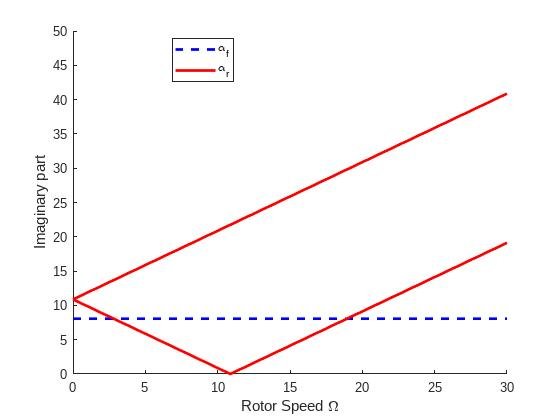
\includegraphics[width=0.7\linewidth]{gambar/Imag(uncoupled).jpg}
	\caption{Plot grafik imajiner terhadap kecepatan rotor $\Omega$ pada kondisi sebelum dimasukkan kondisi \textit{coupled} pada sistem.}
	\label{fig:imag(uncoupled)}
\end{figure}

Pada grafik \ref{fig:imag(uncoupled)} garis putus-putus berwarna biru merupakan nilai eigen untuk \textit{fuselage} helikopter, sehingga pada bagian imajiner tersebut memberikan besarnya mode dari \textit{fuselage}. Sedangkan garis yang berwarna merah merupakan nilai eigen dari mode rotor helikopter, dimana pada grafik tersebut merepresentasikan \textit{regressive rotor mode} dan \textit{progressive rotor mode}. 

\begin{figure}[H]
	\centering
	\includegraphics[width=0.7\linewidth]{gambar/Imag(coupled)_mark.jpg}
	\caption{Plot grafik imajiner terhadap kecepatan rotor $\Omega$ pada kondisi setelah dimasukkan kondisi \textit{coupled} pada sistem.}
	\label{fig:imag(coupled)}
\end{figure}

\begin{figure}[H]
	\centering
	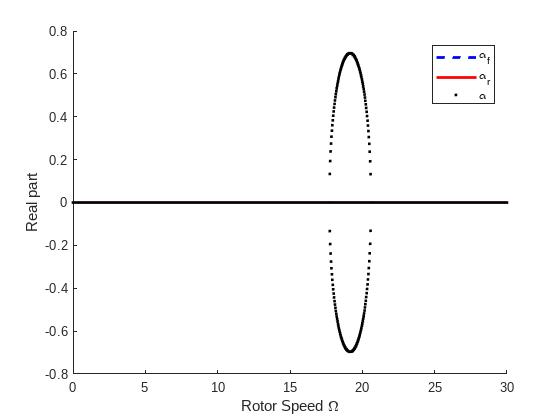
\includegraphics[width=0.7\linewidth]{gambar/Real(coupled).jpg}
	\caption{Plot grafik riil terhadap kecepatan rotor $\Omega$ pada kondisi setelah dimasukkan kondisi \textit{coupled} pada sistem.}
	\label{fig:real(coupled)}
\end{figure}

Grafik pada gambar \ref{fig:imag(coupled)} merupakan grafik saat sistem helikopter yang memiliki interkoneksi pada bagian \textit{input} dan \textit{output} nya (\textit{coupled}). $\alpha$ merupakan nilai eigen dari sistem \textit{coupled}. Kondisi saat nilai eigen \textit{coupled} melebur dengan garis dari nilai eigennya pada nilai eigen di mode \textit{fuselage} nya akan mengakibatkan terjadinya \textit{ground resonance}. Kemudian pada gambar \ref{fig:real(coupled)} memberikan informasi terkait batas siklus osilasi pada satu bilah rotor, yaitu berada pada rentang 17.75-20.57 Hz. Sehingga bila satu buah bilah rotor memiliki frekuensi rotasi pada rentang tersebut, helikopter akan mengalami \textit{ground resonance}.

\begin{figure}[H]
	\centering
	\includegraphics[width=0.7\linewidth]{gambar/sol_plot_2.jpg}
	\caption{Plot solusi gerakan pusat massa rotor pada sumbu-x pada frekuensi rotor 16 Hz.}
	\label{fig:sol_plot_2}
\end{figure}

\begin{figure}[H]
	\centering
	\includegraphics[width=0.7\linewidth]{gambar/sol_plot_3.jpg}
	\caption{Plot solusi gerakan pusat massa rotor pada sumbu-x pada frekuensi rotor 17.75 Hz.}
	\label{fig:sol_plot_3}
\end{figure}

\begin{figure}[H]
	\centering
	\includegraphics[width=0.7\linewidth]{gambar/sol_plot_5.jpg}
	\caption{Plot solusi gerakan pusat massa rotor pada sumbu-x pada frekuensi rotor 30 Hz.}
	\label{fig:sol_plot_5}
\end{figure}

Pada rentang 17.75-20.57 Hz merupakan rentang terjadinya \textit{ground resonance} (gambar \ref{fig:sol_plot_2} hingga \ref{fig:sol_plot_5}). Amplitudo dari solusi perpindahan pusat massa pada sumbu-x berada pada nilai yang besar seiring dengan berjalannya waktu. Hal ini memvalidasi bahwa dalam rentang 17.75-20.57 Hz merupakan rentang terjadinya \textit{ground resonance} helikopter. Amplitudo pada gambar \ref{fig:sol_plot_2} dan \ref{fig:sol_plot_5} memiliki nilai yang berada di skala 0.06 meter. Sedangkan pada gambar \ref{fig:sol_plot_3} amplitudonya membesar seiring berjalannya waktu. 

\begin{figure}[H]
	\centering
	\includegraphics[width=0.75\linewidth]{gambar/xy_2.jpg}
	\caption{Plot pergerakan pusat massa rotor pada sumbu-xy pada frekuensi 16 Hz.}
	\label{fig:xy_2}
\end{figure}

\begin{figure}[H]
	\centering
	\includegraphics[width=0.75\linewidth]{gambar/xy_3.jpg}
	\caption{Plot pergerakan pusat massa rotor pada sumbu-xy pada frekuensi 17.75 Hz.}
	\label{fig:xy_3}
\end{figure}

\begin{figure}[H]
	\centering
	\includegraphics[width=0.75\linewidth]{gambar/xy_5.jpg}
	\caption{Plot pergerakan pusat massa rotor pada sumbu-xy pada frekuensi 30 Hz.}
	\label{fig:xy_5}
\end{figure}

Gambar \ref{fig:xy_2} dan \ref{fig:xy_5} merupakan perpindahan pusat massa rotor helikopter saat tidak terjadi \textit{ground resonance} yaitu pada frekuensi rotor 16 Hz dan 30 Hz. Sedangkan pada gambar \ref{fig:xy_3} merupakan perpindahan pusat massa rotor helikopter saat terjadi fenomena \textit{ground resonance}. Pusat massa rotor seiring berjalannya waktu akan semakin jauh berpindah dari titik pusat massa aslinya, yaitu 0,0, bahkan skala perpindahannya bisa mencapai lebih dari 0.5 meter. 

Gambar pada grafik \ref{fig:real(coupled)} memberikan informasi, bahwa pada bagian riil dari nilai eigen sistem \textit{coupled} berada pada nilai positif pada rentang 17.75-20.57 Hz. Berdasarkan pada apa yang telah dikerjakan pada \cite{BERGEOT201672}, \cite{Eckert2007AnalyticalAA},\cite{Bergeot_passive}, dan banyak literatur mengenai fenomena \textit{ground resonance} maka pada kondisi tersebut helikopter akan mengalami getaran yang dapat menyebabkan \textit{ground resonance}. 

\begin{figure}[H]
	\centering
	\includegraphics[width=0.45\linewidth]{gambar/find_range_10-11,89.png}
	\caption{Jumlah rentang frekuensi respon helikopter pada rentang 17.75-20.57 Hz menggunakan MS Excel.}
	\label{fig:resonance_range}
\end{figure}

Gambar \ref{fig:resonance_range} merupakan langkah yang dilakukan untuk mencari respon helikopter yang terdapat pada interval 17.75-20.57 Hz. Data respon helikopter berada pada A2 hingga A4540. Langkah ini dilakukan untuk mengonfirmasi apakah dari perhitungan matematis, helikopter memiliki potensi mengalami fenomena \textit{ground resonance} atau tidak. Dari hasil tersebut dapat diperhatikan bahwa tidak terdapat respon yang berada pada rentang 17.75-20.57 Hz. Hal ini berkorelasi dengan kondisi di lapangan saat dilakukannya pengujian pada helikopter, bahwa helikopter tidak mengalami getaran besar yang menyebabkan terjadinya \textit{ground resonance}. Aspek penyesuaian yang dipertimbangkan dalam formulasi matematis melibatkan \textit{lagging motion} pada helikopter dan koefisien kopling yang terkuantifikasi secara matematis, sehingga menyebabkan perbedaan nilai pada standar MIL-STD-810H-Method-514.8. Namun, perlu diperhatikan, perhitungan matematis ini didapatkan dengan pendekatan material helikopter yang pada umumnya, yaitu menggunakan material \textit{airframe} helikopter pada umumnya, yaitu Aluminum 7075-T6 \cite{ASTM}.

\subsection{Analisis Matematis Ketidakstabilan Kondisi Modifikasi}

Diasumsikan bahwa pada $m_y$ terdapat penambahan massa baru sebesar $m_m$. Sehingga pada persamaan yang mengandung $m_y$ pada matriks A \ref{eq:state-space} akan menjadi $m'_y$. dengan:

\begin{align}
	\label{eq:modified}
	m'_y=m_y+m_m
\end{align}

Sehingga akan dilakukan perhitungan, saat $m_m = 0$ hingga penambahan sampai pada $m_m = 300$ yang menandakan bahwa perubahan pada massanya akan bertambah sebesar 300 kg. Akan tetapi dalam perhitungan terhadap potensi fenomena \textit{ground resonance} ini memiliki batas penambahan maksimum, yaitu sebesar 4500 kg. Sehingga nilai pertambahan maksimum pada modifikasi helikopter adalah sebesar 2094 kg. Selanjutnya akan coba dilihat melalui grafik seperti pada gambar grafik \ref{fig:imag(coupled)} dan \ref{fig:real(coupled)} untuk kondisi modifikasi penambahan massa pertama, yaitu sebesar 300 kg. Maka akan didapatkan seperti pada gambar \ref{fig:imag(modified)_1} dan \ref{fig:real(modified)_1}.

\begin{figure}[H]
	\centering
	\includegraphics[width=0.65\linewidth]{gambar/imag(modified)_1.jpg}
	\caption{Plot grafik imajiner terhadap kecepatan rotor $\Omega$ pada kondisi \textit{coupled} sebelum (hitam) dan setelah penambahan massa 300 kg (hijau).}
	\label{fig:imag(modified)_1}
\end{figure}

\begin{figure}[H]
	\centering
	\includegraphics[width=0.65\linewidth]{gambar/real(modified)_1.jpg}
	\caption{Plot grafik riil terhadap kecepatan rotor $\Omega$ pada kondisi \textit{coupled} sebelum (hitam) dan setelah penambahan massa 300 kg (hijau).}
	\label{fig:real(modified)_1}
\end{figure}

Variabel keterangan berwarna hijau yang disimbolkan dengan $\alpha_m$ merupakan grafik hasil modifikasi helikopter.  Pada grafik tersebut, yaitu pada gambar \ref{fig:real(modified)_1} dan \ref{fig:imag(modified)_1} menunjukkan adanya pergeseran frekuensi resonansi pada modifikasi penambahan 300 kg pada helikopter, yaitu menjadi 17.45-20.57 Hz. Pergeseran tersebut secara kuantitatif memiliki selisih sebesar 0.3 Hz pada batas awal dan 0.69 Hz batas akhir. Selanjutnya dilakukan penambahan yang lebih berat, yaitu sebesar 1000 kg atau sebesar 1 ton. Sehingga akan didapatkan grafik sebagaimana pada gambar \ref{fig:imag(modified)_2}.

\begin{figure}[H]
	\centering
	\includegraphics[width=0.65\linewidth]{gambar/imag(modified)_2.jpg}
	\caption{Plot grafik imajiner terhadap kecepatan rotor $\Omega$ pada kondisi \textit{coupled} sebelum (hitam) dan setelah penambahan massa 1000 kg (hijau).}
	\label{fig:imag(modified)_2}
\end{figure}

\begin{figure}[H]
	\centering
	\includegraphics[width=0.65\linewidth]{gambar/real(modified)_2.jpg}
	\caption{Plot grafik riil terhadap kecepatan rotor $\Omega$ pada kondisi \textit{coupled} sebelum (hitam) dan setelah penambahan massa 1000 kg (hijau).}
	\label{fig:real(modified)_2}
\end{figure}

Grafik pada gambar \ref{fig:imag(modified)_2} menunjukkan pergeseran rentang frekuensi resonansi yang lebih besar dari sebelumnya. Pada modifikasi penambahan massa 1 ton ini rentang frekuensi resonansi menjadi (16.85-18.68 Hz). Selisih nilai batas awalnya sebesar 0.9 Hz dan batas akhir sebesar 1.89 Hz. Hal ini menujukkan indikasi bahwa modifikasi penambahan massa pada helikopter menggeser rentang frekuensi helikopter ke rentang tertentu. Kemudian selanjutnya dilakukan modifikasi penambahan massa sebesar 2000 kg, penambahan ini secara tidak langsung menjadi batas penambahan maksimal dikarenakan batas beban massa angkat untuk helikopter berdasarkan data \cite{AS565MBe} hanya sebesar 4500 kg.

\begin{figure}[H]
	\centering
	\includegraphics[width=0.65\linewidth]{gambar/imag(modified)_3.jpg}
	\caption{Plot grafik imajiner terhadap kecepatan rotor $\Omega$ pada kondisi \textit{coupled} sebelum (hitam) dan setelah penambahan massa 2000 kg (hijau).}
	\label{fig:imag(modified)_3}
\end{figure}

\begin{figure}[H]
	\centering
	\includegraphics[width=0.65\linewidth]{gambar/real(modified)_3.jpg}
	\caption{Plot grafik riil terhadap kecepatan rotor $\Omega$ pada kondisi \textit{coupled} sebelum (hitam) dan setelah penambahan massa 2000 kg (hijau).}
	\label{fig:real(modified)_3}
\end{figure}

\begin{table}[H]
	\centering
	\caption{Komparasi respon frekuensi pada rentang hasil modifikasi helikopter.}
	\label{tb:respon_modifikasi}
	\resizebox{\textwidth}{!}{%
		\begin{tabular}{|c|c|c|c|}
			\hline
			\begin{tabular}[c]{@{}c@{}}Modifikasi\\ (+ massa) (kg)\end{tabular} & \begin{tabular}[c]{@{}c@{}}Rentang \\ frekuensi (Hz)\end{tabular} & Banyak respon (n) & \begin{tabular}[c]{@{}c@{}}Proporsi dengan seluruh \\ respon frekuensi (\%)\end{tabular} \\ \hline
			300 & 17.45 - 19.88 & 0 & 0\% \\ \hline
			1000 & 16.85 - 18.68 & 0 & 0\% \\ \hline
			2000 & 16.25 - 17.57 & 45 & 2\% \\ \hline
			0-2000 (seluruh rentang) & 16.25 - 20.57 & 45 & 2\% \\ \hline
		\end{tabular}%
	}
\end{table}

Dari grafik \ref{fig:real(modified)_3} menunjukkan pergeseran yang cukup siginifikan untuk rentang frekuensi resonansi helikopter. Untuk modifikasi ini didapatkan rentang pada 16.25-17.57 Hz, dengan selisih batas awal sebesar 1.5 Hz dan batas akhir sebesar 3 Hz. Dari beberapa grafik hasil modifikasi yang telah didapatkan. Modifikasi massa pada helikopter membuat batas siklus osilasinya bergeser ke nilai kecepatan rotor yang lebih rendah. Hal ini disebabkan penambahan massa pada helikopter membuat inersianya juga semakin besar. Sehingga dengan kecepatan yang lebih rendah dari biasanya, sudah cukup untuk membuat helikopter berada pada kondisi yang berpotensi mengalami \textit{ground resonance}. Apabila hasil data akselerometer diidentifikasi pada hasil perhitungan ini dengan rentang keseluruhan dari 16.25 Hz (rentang modifikasi) hingga 20.57 Hz (rentang sebelum dimodifikasi), ditemukan adanya respon pada helikopter pada rentang 16.26-17.57 Hz. Sehingga didapatkan bahwa pada penambahan massa maksimal memiliki sebanyak 45 frekuensi respon atau sebanyak $2\%$ dari total respon helikopter seperti yang ditunjukkan pada tabel \ref{tb:respon_modifikasi}.

Akan tetapi asumsi penambahan massa modifikasi pada helikopter ini didasarkan pada penambahan yang merata pada setiap titik helikopter. Oleh karena itu diperlukan analisis dari aspek geometri jika penambahan massa pada helikopter melibatkan modifikasi bentuk yang tidak merata pada helikopter. Hal tersebut dikarenakan penambahan massa yang tidak merata pada helikopter akan menyebabkan pusat massa helikopter berpindah dari pusat massa awalnya. 


\section{Hasil Pemodelan Simulasi pada Femap}

\subsection{Hasil Femap (\textit{Mode Shape})}



\begin{figure}[H]
	\centering
	\includegraphics[width=0.58\linewidth]{gambar/simulasi_tampak_atas.jpg}
	\caption{Gambar hasil pemodelan stik helikopter tampak dari atas.}
	\label{fig:simulasi_tampak_atas}
\end{figure}

\begin{figure}[H]
	\centering
	\includegraphics[width=0.58\linewidth]{gambar/simulasi_tampak_depan.jpg}
	\caption{Gambar hasil pemodelan stik helikopter tampak dari depan.}
	\label{fig:simulasi_tampak_depan}
\end{figure}

\begin{figure}[H]
	\centering
	\includegraphics[width=0.58\linewidth]{gambar/simulasi_tampak_samping.jpg}
	\caption{Gambar hasil pemodelan stik helikopter tampak dari samping.}
	\label{fig:simulasi_tampak_samping}
\end{figure}

\begin{figure}[H]
	\centering
	\includegraphics[width=0.58\linewidth]{gambar/simulasi_tampak_normal.jpg}
	\caption{Gambar hasil pemodelan stik helikopter tampak dari normal.}
	\label{fig:simulasi_tampak_normal}
\end{figure}

Hasil simulasi pada Femap menggunakan beberapa kondisi pendekatan dengan keadaan sebenarnya dari helikopter. Dalam hal ini, diberikan \textit{constraint} pada beberapa titik di helikopter. Titik tersebut terletak pada bagian depan dan tengah diposisi kanan-kiri kerangka helikopter. \textit{Constraint} tersebut merepresentasikan posisi pendaratan helikopter pada darat, yaitu ban dan oleo. Dari titik yang telah ditentukan pada tabel \ref{tb:koordinat}, yaitu terletak pada ID 9, 10, 15, dan 16 atau jika dilihat menggunakan skema pada gambar \ref{fig:skema_model} terletak pada mark 1s, 1s', 3s dan 3s'. \textit{Constraint} yang diberikan merupakan batasan yang hanya berada pada arah sumbu-x. Sehingga pada titik tersebut tidak terdapat perindahan secara translasi.

Helikopter dimodelkan berdasarkan model stik atau batang. Pada masing-masing penghubung stiknya merupakan \textit{node}. Digunakan material berbahan dasar aluminum 7075-T6 untuk elemen pada stik pemodelan helikopter dengan informasi yang didapat dari \cite{ASTM}.

Dari pemodelan yang telah dibuat pada Femap, selanjutnya telah digunakan analisis pada fitur Femap untuk mencari \textit{mode shape} pada helikopter. Secara matematis, pada dasarnya untuk mencari \textit{mode shape} pada helikopter adalah dengan mencari nilai eigen dari sistem pemodelannya. Kemudian dari nilai eigen tersebut didapatkan vektor eigen untuk selanjutnya dapat merepresentasikan gerakan dari n-mode yang dimilki oleh helikopter. Dalam hal ini telah didapatkan 10 mode pada helikopter.

Pada gambar \ref{fig:mode1} hingga \ref{fig:mode10} merupakan deformasi mode 1 hingga mode 10. Setiap mode memiliki bentuk deformasi dan frekuensi yang berbeda-beda. Mode 1 hingga 3 memiliki frekuensi yang sangat kecil, dari ketiga \textit{mode shape} tersebut memiliki gerakan yang hampir sama. Kemudian pada mode 4 hingga 10 memiliki frekuensi dan \textit{mode shape} yang berbeda-beda pula. Bila dikembalikan pada pemahaman teoritis, fenomena \textit{ground resonance} dapat terjadi apabila peredam pada bilah rotor tidak dapat mengkompensasi gerakan tertinggal bilahnya (\textit{lead/lag motion}) maka pusat massa helikopter tidak akan segaris lagi dengan rotor. Hal tersebut dapat menyebabkan ketidakstabilan oleh gaya sentrifugal (gambar \ref{fig:simulasiGR}) pada frekuensi tertentu yang menyebabkan badan helikopter mengalami getaran dan saat frekuensi dari rotor memiliki nilai yang mendekati frekuensi natural helikopter maka terjadilah \textit{ground resonance}.

\begin{figure}[H]
	\begin{subfigure}{0.49\textwidth}
		\centering
		\includegraphics[width=0.9\linewidth]{gambar/mode1.jpg}
		\caption{}
		\label{fig:mode1}
	\end{subfigure}
	\centering
	\begin{subfigure}{0.49\textwidth}
		\centering
		\includegraphics[width=0.9\linewidth]{gambar/mode2.jpg}
		\caption{}
		\label{fig:mode2}
	\end{subfigure}
	\caption{Deformasi pada: (a) mode 1 di frekuensi 4.12*$10^-6$ Hz (b) mode 2 di frekuensi 1.07*$10^-6$ Hz.}
	\label{fig:modeshape1}
\end{figure}

\begin{figure}[H]
	\begin{subfigure}{0.49\textwidth}
		\centering
		\includegraphics[width=0.9\linewidth]{gambar/mode3.jpg}
		\caption{}
		\label{fig:mode3}
	\end{subfigure}
	\centering
	\begin{subfigure}{0.49\textwidth}
		\centering
		\includegraphics[width=0.9\linewidth]{gambar/mode4.jpg}
		\caption{}
		\label{fig:mode4}
	\end{subfigure}
	\caption{Deformasi: (a) mode 3 pada frekuensi 1.34*$10^-6$ Hz (b) mode 4 pada frekuensi 2.73 Hz.}
\end{figure}

\begin{figure}[H]
	\begin{subfigure}{0.49\textwidth}
		\centering
		\includegraphics[width=0.9\linewidth]{gambar/mode5.jpg}
		\caption{}
		\label{fig:mode5}
	\end{subfigure}
	\centering
	\begin{subfigure}{0.49\textwidth}
		\centering
		\includegraphics[width=0.9\linewidth]{gambar/mode6.jpg}
		\caption{}
		\label{fig:mode6}
	\end{subfigure}
	\caption{Deformasi: (a) mode 5 pada frekuensi 2.74 Hz (b) mode 6 pada frekuensi 4.31 Hz.}
\end{figure}

\begin{figure}[H]
	\begin{subfigure}{0.49\textwidth}
		\centering
		\includegraphics[width=0.9\linewidth]{gambar/mode7.jpg}
		\caption{}
		\label{fig:mode7}
	\end{subfigure}
	\centering
	\begin{subfigure}{0.49\textwidth}
		\centering
		\includegraphics[width=0.9\linewidth]{gambar/mode8.jpg}
		\caption{}
		\label{fig:mode8}
	\end{subfigure}
	\caption{Deformasi: (a) mode 7 pada frekuensi 6.17 Hz (b) mode 8 pada frekuensi 7.31 Hz.}
\end{figure}

\begin{figure}[H]
	\begin{subfigure}{0.49\textwidth}
		\centering
		\includegraphics[width=0.9\linewidth]{gambar/mode9.jpg}
		\caption{}
		\label{fig:mode9}
	\end{subfigure}
	\centering
	\begin{subfigure}{0.49\textwidth}
		\centering
		\includegraphics[width=0.9\linewidth]{gambar/mode10.jpg}
		\caption{}
		\label{fig:mode10}
	\end{subfigure}
	\caption{Deformasi: (a) mode 9 pada frekuensi 10.1 Hz (b) mode 10 pada frekuensi 10.7 Hz.}
	\label{fig:modeshape10}
\end{figure}

\begin{figure}[H]
	\centering
	\includegraphics[width=0.7\linewidth]{gambar/simulasiGR.png}
	\caption{Gaya sentrifugal dan ketidakstabilan helikopter saat \textit{ground resonance}.}
	\label{fig:simulasiGR}
\end{figure}

Dari beberapa \textit{mode shape} yang telah didapatkan, terdapat salah satu gerakan pada \textit{mode shape} yang memiliki bentuk yang serupa dengan fenomena pada gambar \ref{fig:simulasiGR}, yaitu pada mode ke-6. Pada mode tersebut, \textit{fuselage} memiliki getaran yang bergerak pada sumbu-y (kanan-kiri).

\begin{figure}[H]
	\begin{subfigure}{0.49\textwidth}
		\centering
		\includegraphics[width=0.9\linewidth]{gambar/mode6_frame_1.PNG}
		\caption{}
		\label{fig:mode6_frame_1}
	\end{subfigure}
	\centering
	\begin{subfigure}{0.49\textwidth}
		\centering
		\includegraphics[width=0.9\linewidth]{gambar/mode6_frame_2.PNG}
		\caption{}
		\label{fig:mode6_frame_2}
	\end{subfigure}
	\caption{Gerakan pada mode ke-6 saat: (a) animasi frame ke-1 (b) animasi frame ke-2.}
\end{figure}

\begin{figure}[H]
	\begin{subfigure}{0.49\textwidth}
		\centering
		\includegraphics[width=0.9\linewidth]{gambar/mode6_frame_3.PNG}
		\caption{}
		\label{fig:mode6_frame_3}
	\end{subfigure}
	\centering
	\begin{subfigure}{0.49\textwidth}
		\centering
		\includegraphics[width=0.9\linewidth]{gambar/mode6_frame_4.PNG}
		\caption{}
		\label{fig:mode6_frame_4}
	\end{subfigure}
	\caption{Gerakan pada mode ke-6 saat: (a) animasi frame ke-3 (b) animasi frame ke-4.}
\end{figure}

Dalam pemodelan simulasi pada Femap, terdapat banyak aspek yang disederhanakan. Bentuk helikopter yang sangat kompleks direpresentasikan dalam bentuk stik model seperti yang dikerjakan pada \cite{Grzegorz2016THESP} dimana pada pemodelan tersebut, digunakan data propertis yang sudah sesuai dengan kondisi eksisting pada helikopter. Akan tetapi pada pemodelan yang telah dibuat kali ini, masih menjadi sebuah batasan untuk melakukan pendekatan sesuai dengan propertis material yang digunakan. Sehingga pada pemodelan ini hanya akan digunakan analisis untuk merepresentasikan \textit{mode shape} yang sesuai dengan mekanisme terjadinya fenomena \textit{ground resonance}.

\begin{figure}[h]
	\centering
	\includegraphics[width=0.94\linewidth]{gambar/find_femap_range}
	\caption{Jumlah rentang respon frekuensi hasil simulasi Femap pada rentang 4-4.5 Hz menggunakan MS Excel.}
	\label{fig:fem_range}
\end{figure}


Frekuensi pada mode ke-6, merupakan frekuensi eigen yang berada dekat pada rentang frekuensi $f_1$ (5.92-6.02 Hz). Apabila pada rentang frekuensi di mode ke-6 dilakukan identifikasi jumlah frekuensi respon helikopter seperti yang dapat dilihat pada gambar \ref{fig:fem_range}, akan didapatkan sebanyak $3\%$ respon frekuensi helikopter yang berada pada sekitar frekuensi mode ke-6 (82 respon frekuensi) dengan batas-batas pada 4-4.5 Hz. Hal ini mnunjukkan, bahwa apabila ditinjau dari \textit{finite element analysis}, tidak terdapat potensi yang besar untuk terjadinya fenomena \textit{ground resonance} pada helikopter hasil modifikasi ini. 

\subsection{Validasi Hasil Simulasi}

Validasi simulasi yang dilakukan berdasarkan pada deformasi pada hasil \textit{mode shape} simulasi Femap. Dari data pengukuran, sensor akselerometer diletakkan pada titik 2s', 2s, dan 3s'. Kemudian selanjutnya akan dilakukan identifikasi deformasi pada titik 3s' pada arah sumbu-y seperti yang dapat dilihat pada gambar \ref{fig:FEM_pengukuran}.

Deformasi pada titik 3s' (node ke-15) di mode-6 (4.31 Hz) pada arah sumbu-y didapatkan sebesar 0.016 m. Sehingga bila diekspresikan dalam bentuk getaran (gambar \ref{fig:fem_validation_time_domain}) akan dihasilkan grafik perbandingan perpindahan hasil pengukuran pada titik 3s' terhadap simulasi Femap. Selanjutnya dari hasil FFT untuk kedua respon frekuensi (pengukuran dan simulasi) didapatkan dari hasil simulasi frekuensinya berada pada 9.30 Hz. Sedangkan untuk hasil pengukuran sebesar 16.19. Sehingga terhadap dominan frekuensinya didapatkan besarnya error antara keduanya adalah sebesar 42.5$\%$ sedangkan untuk \textit{root mean square error} nya didapatkan sebesar 5.8$\%$. 

\begin{figure}[H]
	\centering
	\includegraphics[width=0.9\linewidth]{gambar/FEM.png}
	\caption{Bentuk \textit{finite element} stik model pada titik pengukuran helikopter.}
	\label{fig:FEM_pengukuran}
\end{figure}

\begin{figure}[H]
	\centering
	\includegraphics[width=0.9\linewidth]{gambar/fem_compare.jpg}
	\caption{Respon frekuensi helikopter pada arah sumbu-x dan Plot simulasi Femap arah sumbu-x.}
	\label{fig:fem_validation_time_domain}
\end{figure}

\begin{figure}[H]
	\centering
	\includegraphics[width=0.8\linewidth]{gambar/fem_fft.jpg}
	\caption{Respon frekuensi helikopter pada arah sumbu-x dan Plot simulasi Femap arah sumbu-x.}
	\label{fig:fem_fft}
\end{figure}

Hasil simulasi yang didapatkan memiliki nilai error yang cukup besar dari hasil pengukuran. Meskipun identifikasi dari gerakan hasil simulasi memiliki gerakan yang serupa dengan fenomena \textit{ground resonance}. Akan tetapi secara kuantitatif, nilai tersebut memiliki error yang hampir mencapai 42.5$\%$. Error tersebut dapat disebabkan oleh pendekatan propertis mekanik yang belum sesuai dengan helikopter yang sebenarnya dan pembuatan \textit{finite element} yang masih belum sesuai dengan model stik helikopter. Sehingga pada skala pengembangan kedepannya diperlukan bentuk \textit{finite element} yang lebih akurat dan pemilihan propertis mekanik yang lebih sesuai dengan helikopter yang dimodelkan.